\subsection{Peak Utilization}
\label{subsec:peak-util}

% We shed light on the user's and ISP's \textbf{differing perspectives of \emph{capacity utilization}}, and show that indeed, the user's behavior does change when offered a higher capacity link even though the overall utilization stops increasing after a certain upper limit.

\hypoth{2}. Does the maximum (or 90-\%ile) data transferred by the device differ?

\begin{itemize}
\itemsep0em 
\item Figure ~\ref{fig:CDF-data-rate-max}
\item Calculate the maximum data rate for a device over the three months, and compare max rate (per device) for test set and max rate (per device) for control set
\item test set has higher (max) average data rate below 10 kbps \todo{sanity check numbers, redo plot}
\item 30\% of devices in the control set have a max data rate of 2 kbps while 30\% of test set has a max data rate of 10 kbps.
\end{itemize}

%%%%%%%%%%%%%%%%%%%%%%%%%%%%%%%%%%%%%%%%%%%%%%%%%%%%%%%%%%%%%%%%%%%%%
\begin{figure}[ht!]
%\hspace*{-0.2in}
\begin{minipage}{0.90\linewidth}
\centering
%
%\hfill
\begin{subfigure}[b]{0.90\linewidth}
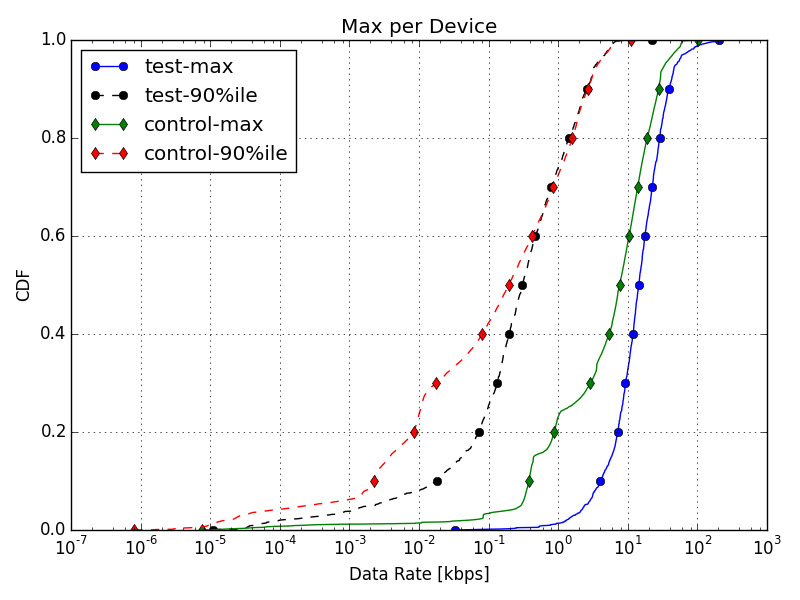
\includegraphics[width=\linewidth]{figures/cdf-max-per-device.png}
  \caption{CDF of max per device}
  %http://sites.noise.gatech.edu/~sarthak/files/comcast/plots/full_dw/cdf-max-per-device.png
  \label{fig:CDF-data-rate-max}
\end{subfigure}
%
\vspace{-1em}
%
\begin{subfigure}[b]{0.90\linewidth}
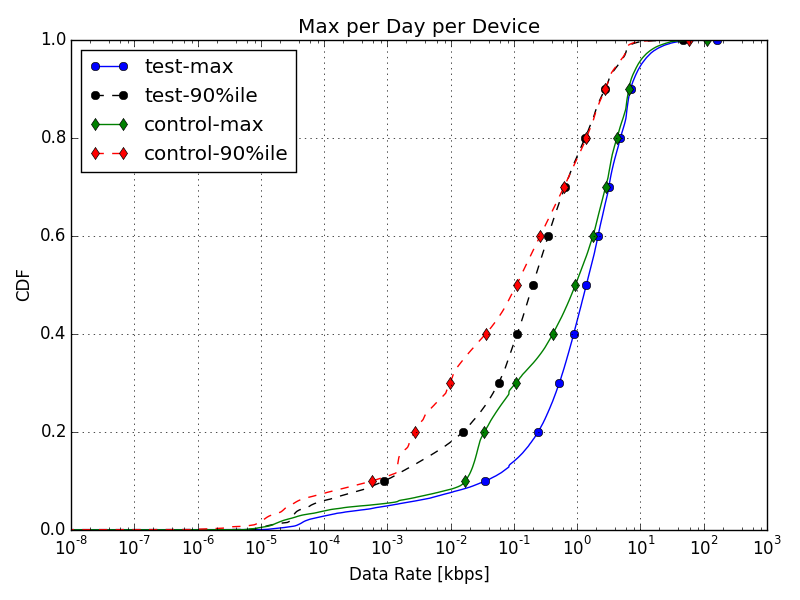
\includegraphics[width=\linewidth]{figures/cdf-max-per-day-per-device.png}
  \caption{CDF of max per device daily}
  \vspace{1em}
  %http://sites.noise.gatech.edu/~sarthak/files/comcast/plots/full_dw/cdf-max-per-day-per-device.png
  \label{fig:CDF-data-rate-max-daily}
\end{subfigure}
%\hfill
\end{minipage}
\caption{Peak Utilization: The maximum data rate varies for test and control set for low data rates, and this variation is present daily.}
\label{fig:peak-utilization}
% created using docs/metadata-separated.log
\end{figure}
%%%%%%%%%%%%%%%%%%%%%%%%%%%%%%%%%%%%%%%%%%%%%%%%%%%%%%%%%%%%%%%%%%%%%

\begin{itemize}
\itemsep0em 
\item Figure ~\ref{fig:CDF-data-rate-max-daily}
\item Max seen by a device per day, in 3 months
\item Consistent increase for daily max data rate per device
\item 15 min granularity misses information
	\begin{itemize}
	\itemsep0em
	\item short faster data bursts
	\item better video quality
	\item baseline is different
	\end{itemize}
\end{itemize}


%------------------------------------------------------------------------------

\begin{figure}[b]{0.90\linewidth}
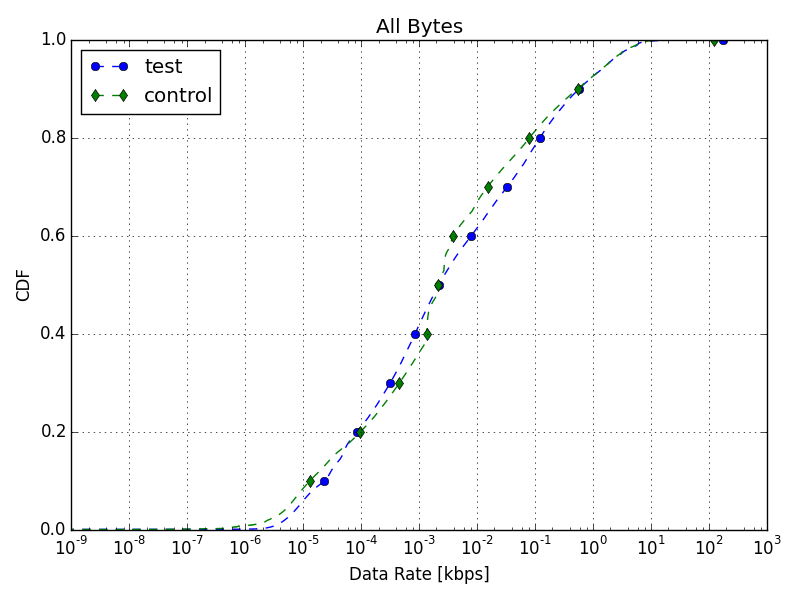
\includegraphics[width=\linewidth]{figures/cdf-all-bytes.png}
  \caption{CDF of data rate per time slot for all devices (agg view of data): Overall not much change due to capacity increase}
  \vspace{1em}
  %http://sites.noise.gatech.edu/~sarthak/files/comcast/plots/full_dw/cdf-all-bytes.png
  \label{fig:CDF-data-rate-all}
\end{figure}
%\hfill

\begin{itemize}
\itemsep0em 
\item Figure ~\ref{fig:CDF-data-rate-all}
\item Distribution of average data rate (kbps) per 15-min time slot 
\item Very similar distributions of bytes transferred
\item Median data rate ~ 2bps for 3 months x thousands of devices!
\end{itemize}
